% !TeX root = ../../beamer.tex
\section{Geschichte}

\begin{frame}
    \frametitle{Das Daventry Experiment}

    \begin{columns}
        \begin{column}{0.5\textwidth}
            \begin{itemize}
                \item \textbf{Passives} Radar
                \item BBC Sendeturm als Beleuchter
                \item Detektion von Bomber-Flugzeug
            \end{itemize}
        \end{column}
        \begin{column}{0.5\textwidth}
            \begin{figure}
                \centering
                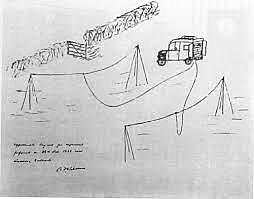
\includegraphics[height=5cm]{daventry_experiment.jpg}
                \caption{Skizze des Daventry Experiments von 1935~\cite{WattsonWatt1935}.}
            \end{figure}
        \end{column}
    \end{columns}
\end{frame}

\begin{frame}
    \frametitle{Chain Home}

    \begin{columns}
        \begin{column}{0.5\textwidth}
            \begin{itemize}
                \item Aktives Radar
                \item Nutzung während des 2. Weltkriegs
                \item Frühwarnradar gegen deutsche Luftangriffe
                \item Erste Inbetriebnahme 1937
            \end{itemize}
        \end{column}
        \begin{column}{0.5\textwidth}
            \begin{figure}
                \centering
                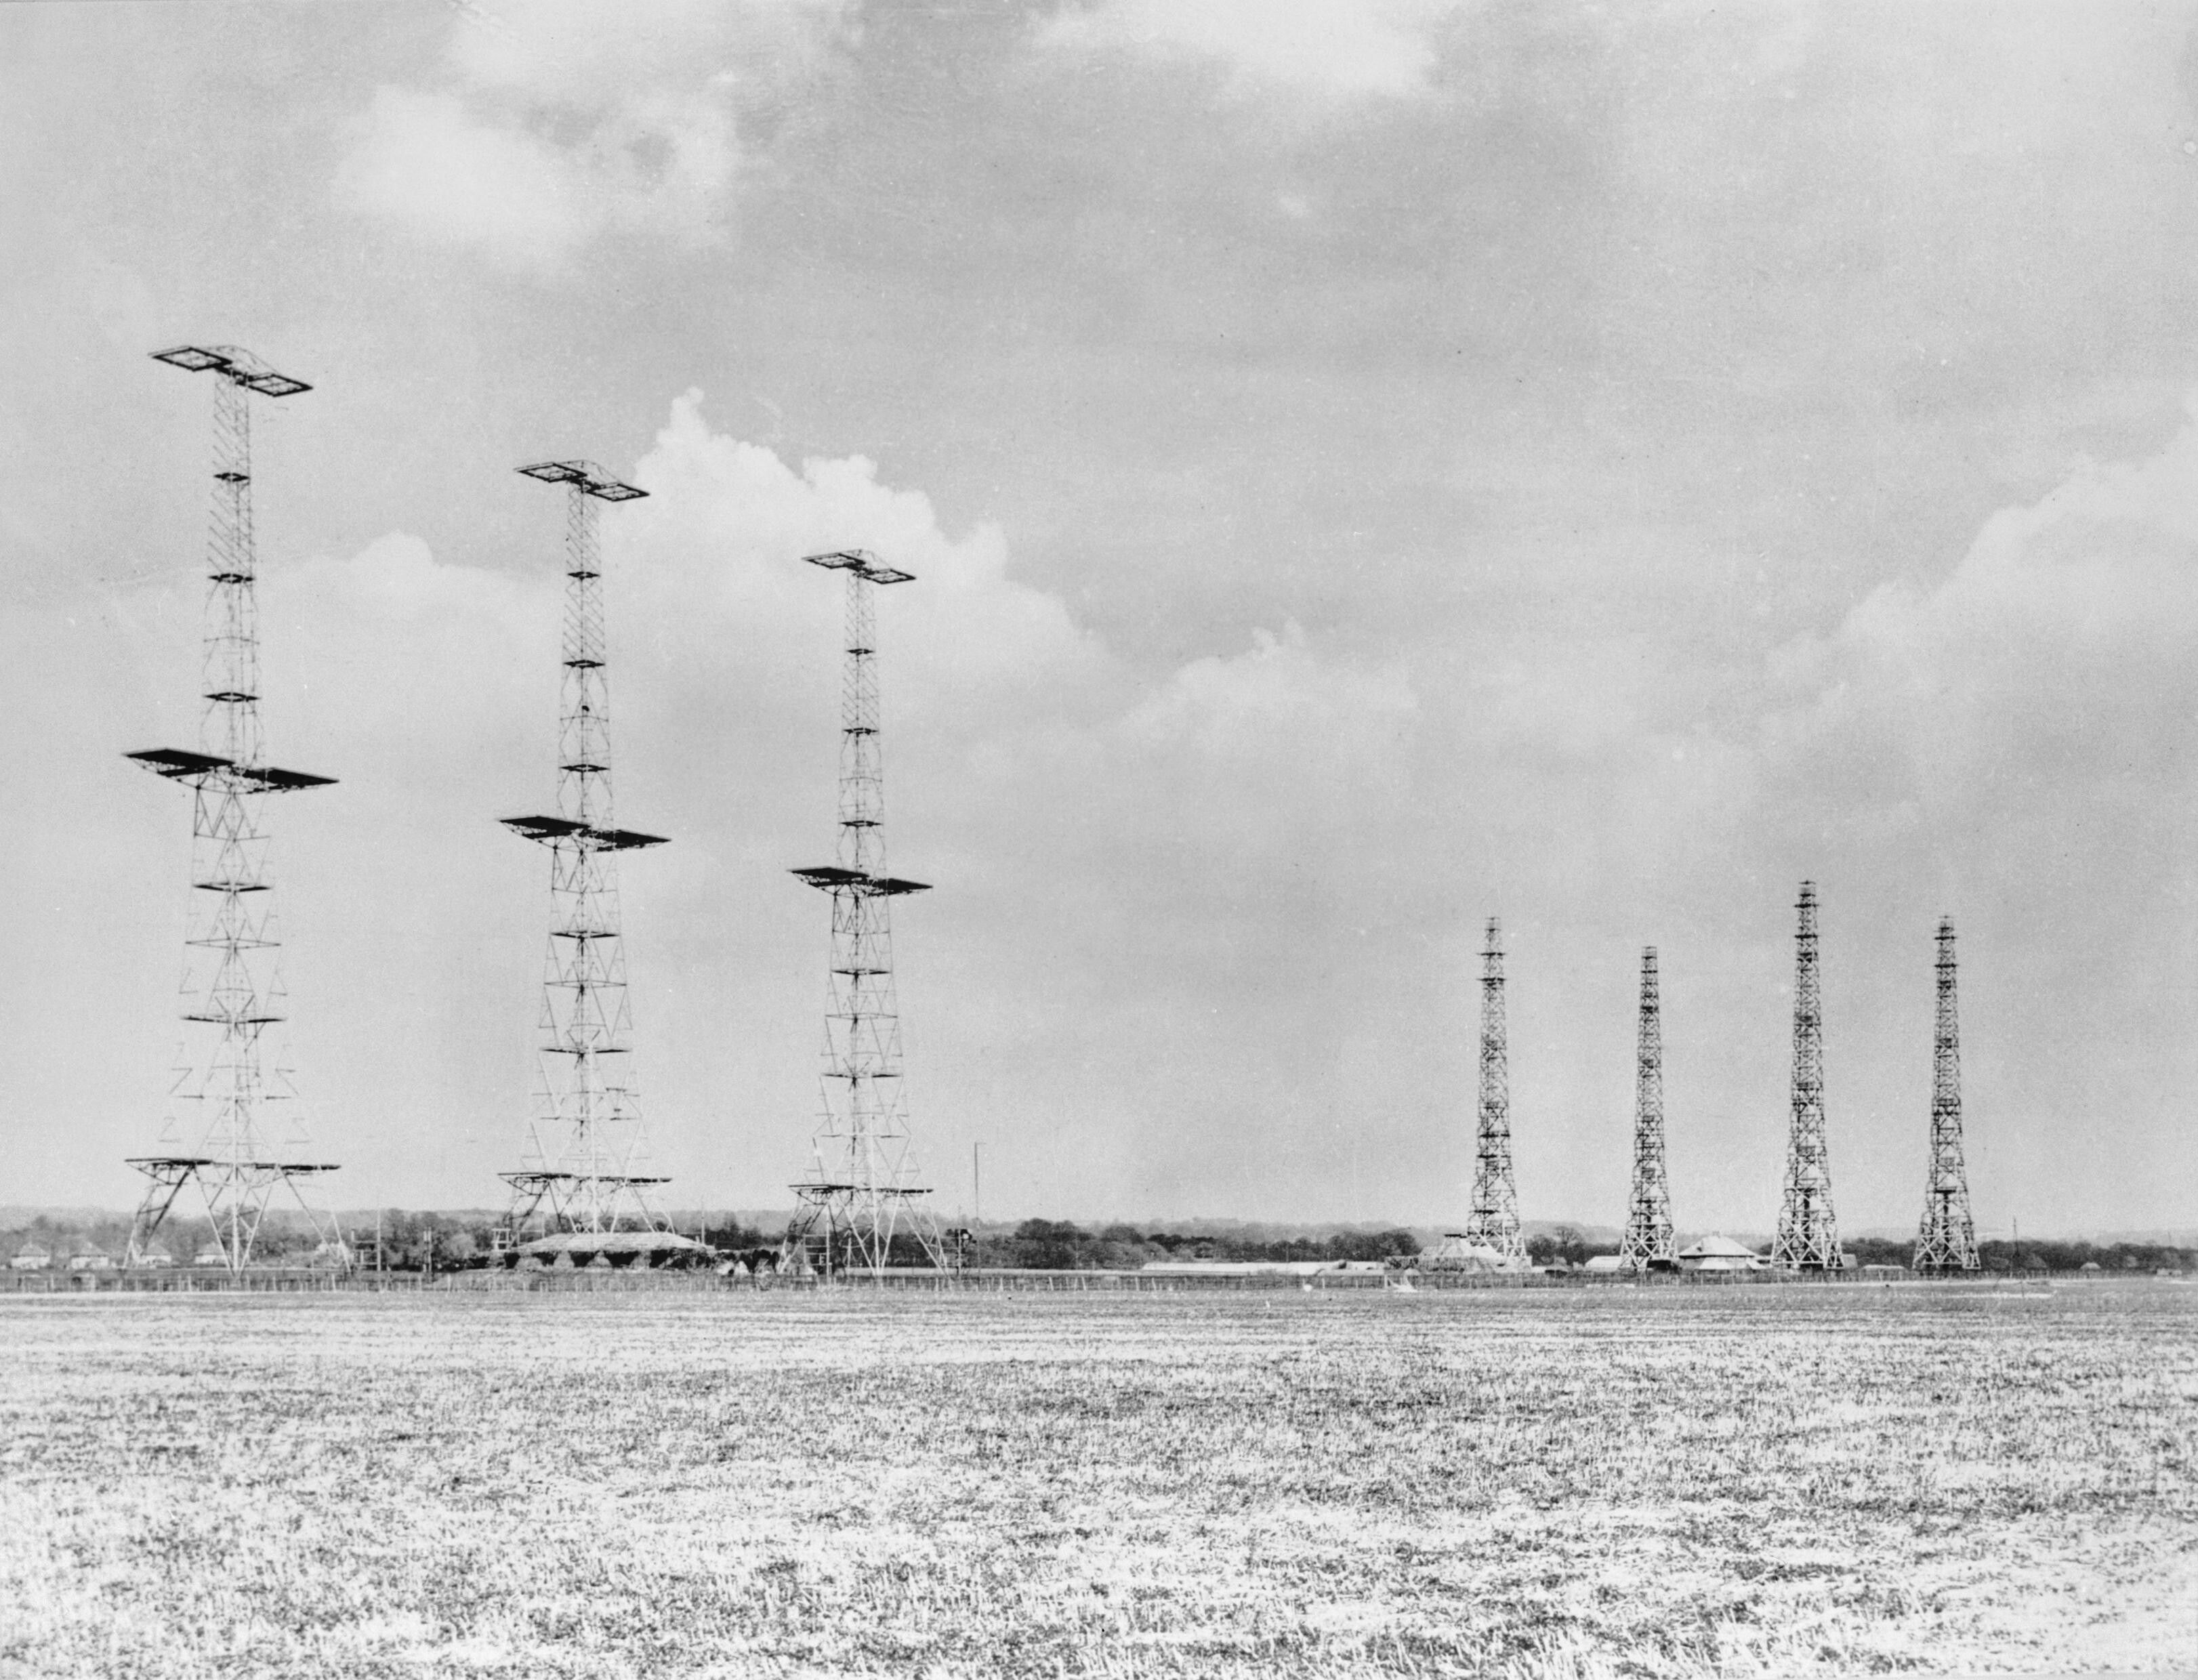
\includegraphics[height=5cm]{chain_home.jpg}
                \caption{Chain Home Antennen der Royal Airforce. Foto 1945~\cite{RoyalAirForce1945}.}
            \end{figure}
        \end{column}
    \end{columns}
\end{frame}

\begin{frame}
    \frametitle{Klein Heidelberg}

    \begin{columns}
        \begin{column}{0.44\textwidth}
            \begin{figure}
                \centering
                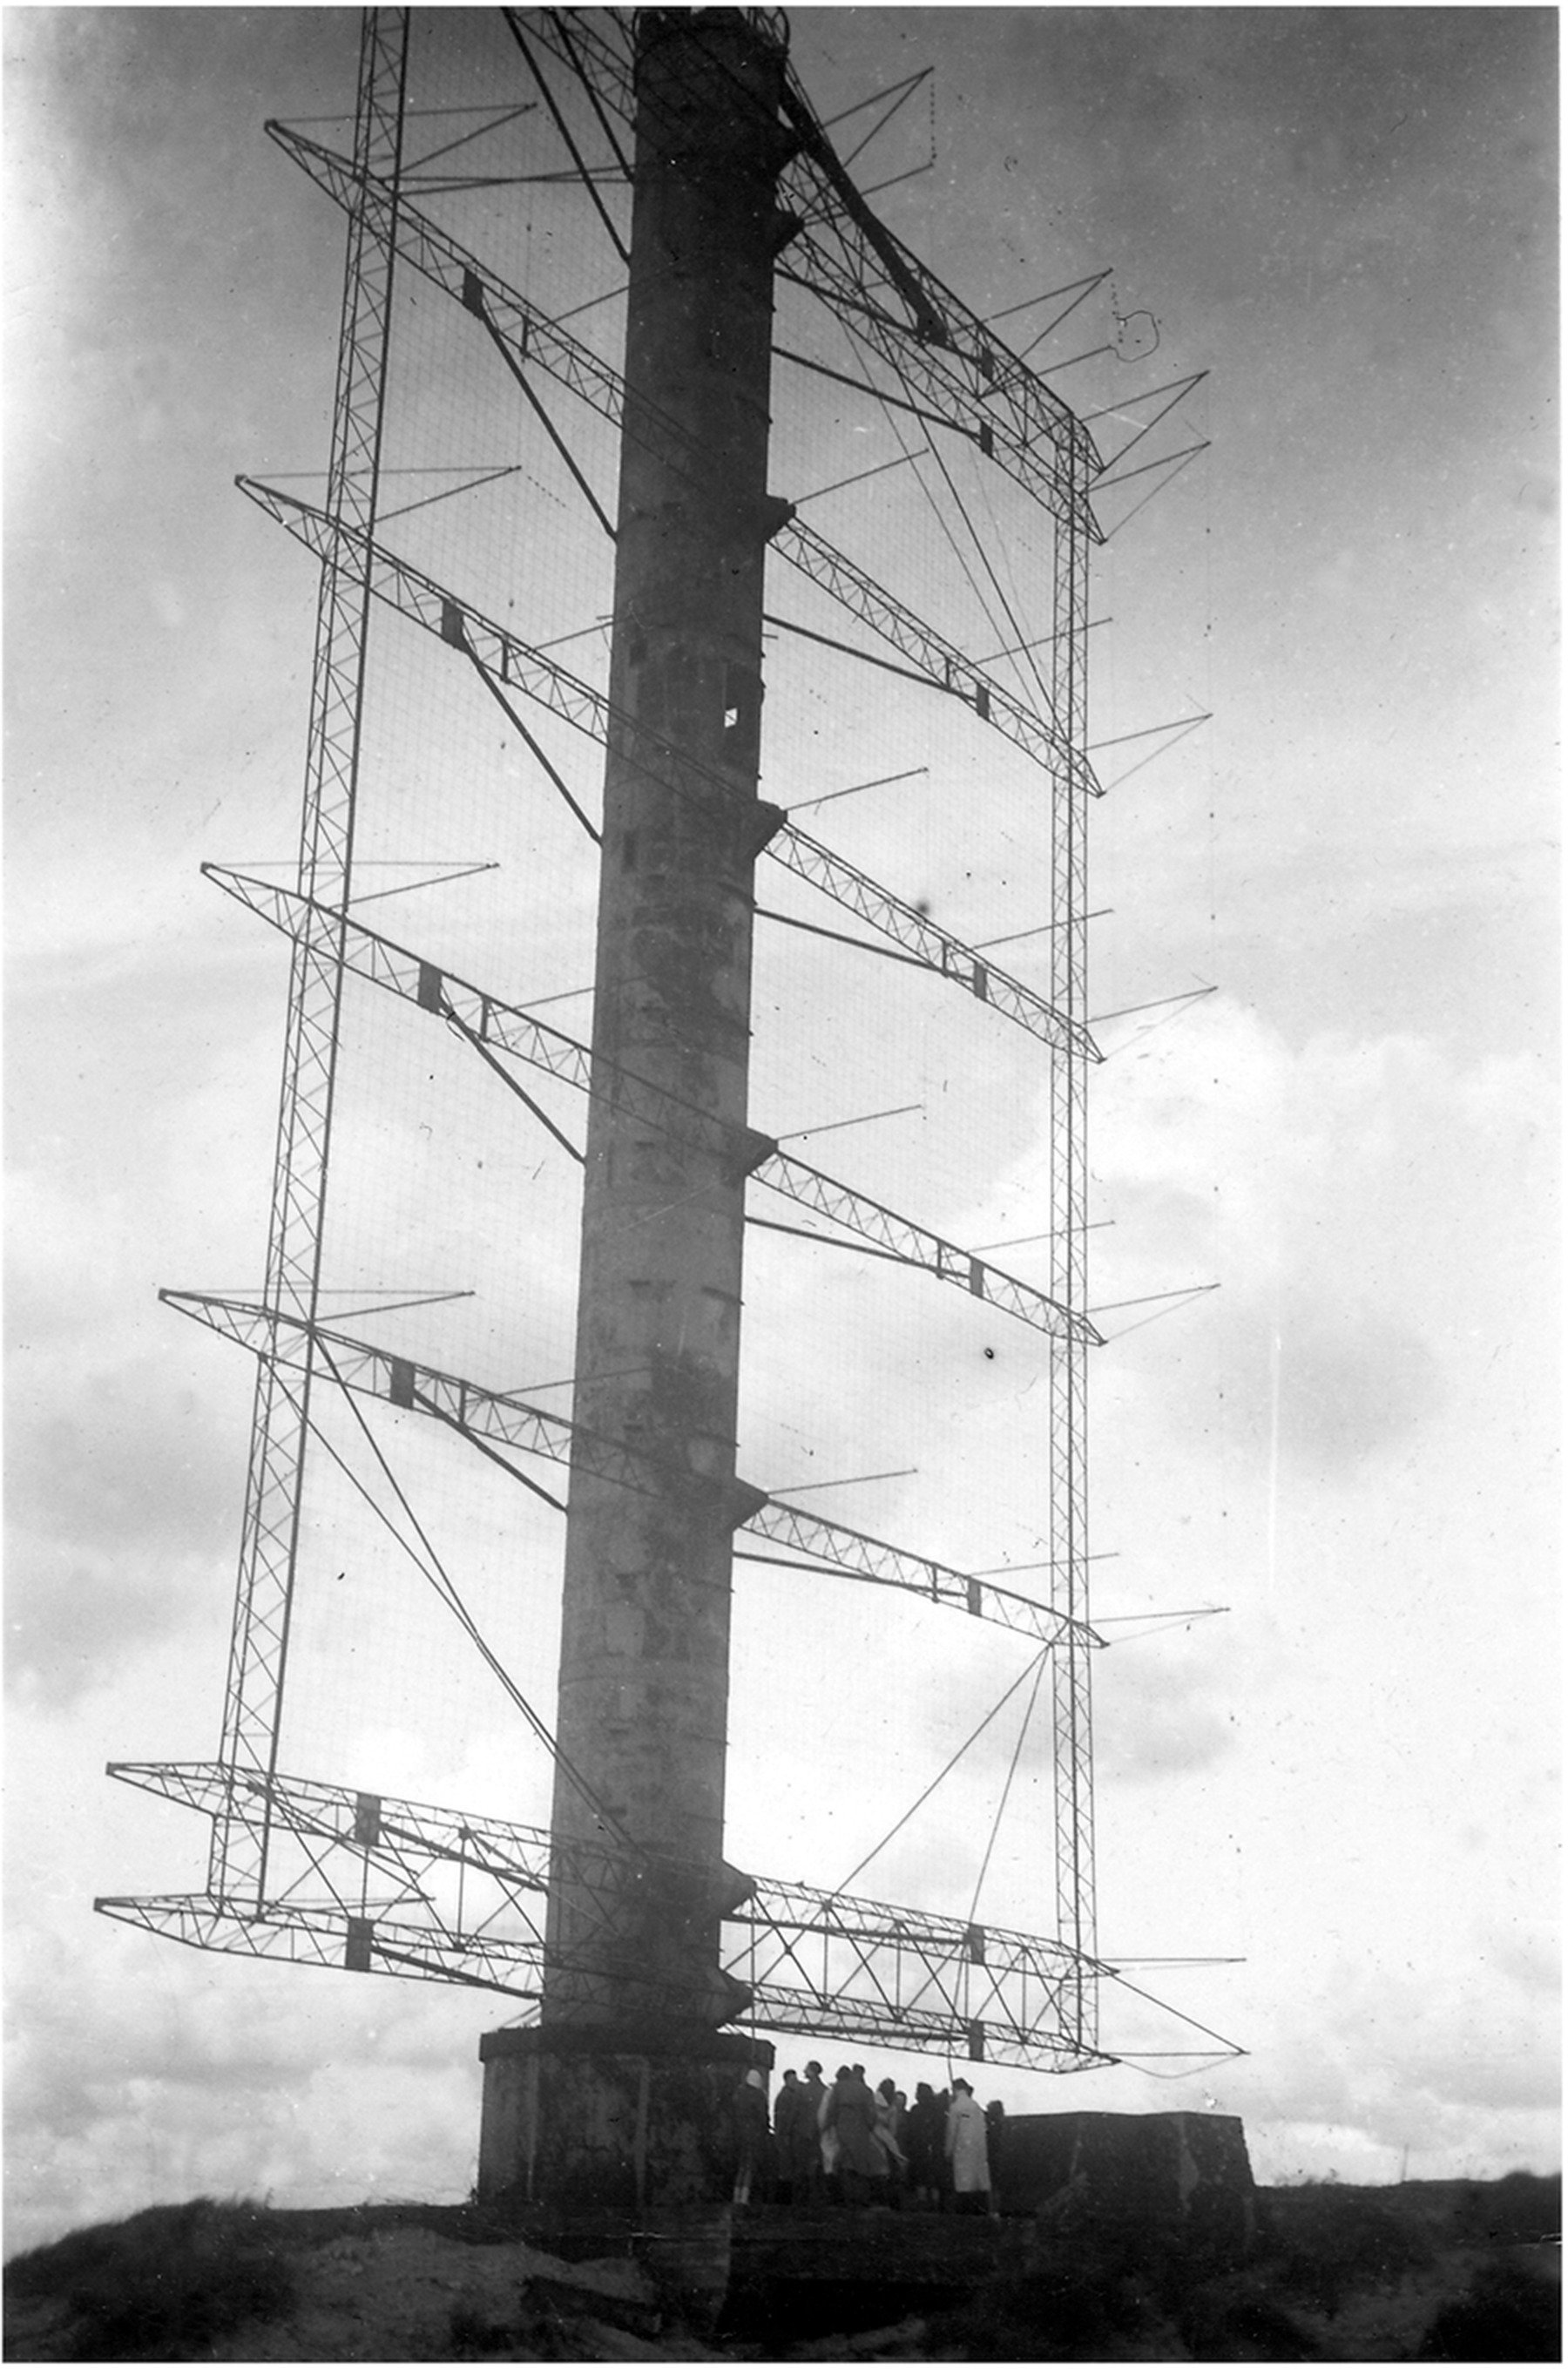
\includegraphics[height=4.5cm]{klein_heidelberg.jpg}
                \caption{Antenne des Klein Heidelberg Empfängers BIEBER (Oostvoorne, NL). Foto 1947~\cite{Rijpsma2005} as cited in~\cite{Griffiths2010}.}
            \end{figure}
        \end{column}
        \begin{column}{0.56\textwidth}
            \begin{itemize}
                \item \textbf{Passives} Radar
                \item Detektion von britischen Bombern über dem Ärmelkanal
                \item Nutzte \textbf{britisches Chain-Home} als Beleuchter
                \item Fertigstellung 1942
            \end{itemize}
        \end{column}
    \end{columns}
\end{frame}

\begin{frame}
    \frametitle{Neuzeit}

    \begin{columns}
        \begin{column}{0.55\textwidth}
            \begin{figure}
                \centering
                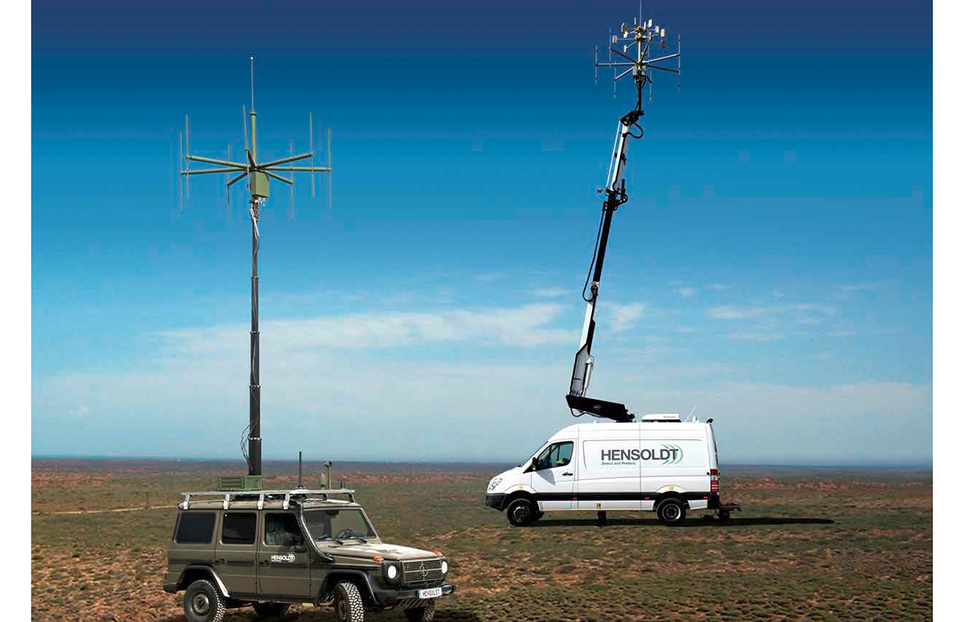
\includegraphics[height=4.75cm]{twinvis.png}
                \caption{TwInvis®. Modernes Passivradarsystem des Unternehmens Hensoldt~\cite{Hensoldt2019}.}
            \end{figure}
        \end{column}
        \begin{column}{0.45\textwidth}
            \begin{itemize}
                \item Zunächst basierend auf FM Beleuchtern
                \item Später DAB und DVB-T
                \item GSM, LTE
                \item \dots
            \end{itemize}
        \end{column}
    \end{columns}
\end{frame}
